\documentclass[11pt]{article}

\usepackage[margin=1in]{geometry}
\usepackage{graphicx}
\usepackage{amsmath}
\usepackage{booktabs}
\usepackage{setspace}
\usepackage{authblk}
\usepackage[authoryear,colon,sort]{natbib}
\usepackage{hyperref}

\title{Compositional and Dynamical Metrics of Cortical Organization:\\Alignment with the Principal Cortical Gradient}

\author[1]{Mark Rowe Traver}
\affil[1]{Independent Researcher}

\date{April 2026}

\begin{document}

\maketitle

\begin{abstract}
	We examine two complementary metrics of cortical organization derived from representational data. First, we introduce the Composite Dispersion Index (CDI), defined as the product of activation magnitude, variance, and standard deviation. Second, we define a dynamical torsion metric ($\chi$) inspired by the SFH-SGP framework, computed as the Frobenius norm of the antisymmetric component of the estimated Jacobian of velocity with respect to state. Using TRIBE v2 model predictions mapped to Schaefer-400 parcels ($n = 400$), we find that CDI shows weak positive correlation with the cortical gradient ($r = 0.104$, $p = 0.038$), while $\chi$ shows stronger negative correlation ($r = -0.183$, $p < 10^{-3}$). Critically, $\chi$ maintains significant partial correlation after controlling for norm ($r = -0.297$, $p < 10^{-8}$), demonstrating that the dynamical torsion measure captures variance beyond simple magnitude or dispersion. Both metrics survive spatial spin permutation testing. These findings suggest that both compositional and dynamical aspects of representational geometry align with cortical hierarchy.
\end{abstract}

\textbf{Keywords:} Cortical Gradient, CDI, Dynamical Torsion, SFH-SGP, Cortical Organization, Schaefer-400

\section{Introduction}

The principal cortical gradient from \citet{Margulies2016} provides a fundamental coordinate system for cortical hierarchy, ranging from primary sensory/motor regions to transmodal association cortex. Understanding what representational properties align with this gradient illuminates the organizing principles of cortical function.

In this study, we examine two complementary aspects of representational geometry:

\begin{enumerate}
	\item \textbf{Composite Dispersion Index (CDI)}: A nonlinear combination of activation magnitude and dispersion that captures the overall ``spread'' of representational patterns.
	\item \textbf{Dynamical Torsion ($\chi$)}: A measure inspired by the SFH-SGP (Sentient Field Hypothesis -- Stochastic Geometric Process) framework that captures the rotational (antisymmetric) component of estimated dynamics.
\end{enumerate}

We emphasize that this is not a validation of the SFH-SGP theory. Rather, we test whether a dynamical torsion-like quantity inspired by the framework shows meaningful alignment with cortical organization.

\section{Theoretical Background}

\subsection{Composite Dispersion Index (CDI)}

The CDI is defined as:

\[
	\text{CDI} = \|x\| \cdot \text{Var}(x) \cdot \text{Std}(x)
\]

This metric captures the overall ``dispersiveness'' of activation patterns. It is explicitly a nonlinear combination of magnitude and variance measures, not a dynamical quantity.

\subsection{Dynamical Torsion ($\chi$)}

The SFH-SGP framework proposes that reality emerges from stochastic interaction processes, with dynamics characterized by torsional flow. While we do not claim to measure the theoretical quantity $\chi$, we define an operationalization:

For a time series $x_t$:

\begin{enumerate}
	\item \textbf{Velocity}: $v_t = x_{t+1} - x_t$
	\item \textbf{Jacobian estimation}: $J = \text{Cov}(v, x) \cdot \text{Cov}(x, x)^{-1}$
	\item \textbf{Antisymmetric component}: $A = (J - J^T) / 2$
	\item \textbf{Torsion}: $\chi = \|A\|_F$ (Frobenius norm)
\end{enumerate}

This metric specifically captures the rotational (non-conservative) component of estimated dynamics. Unlike CDI, $\chi$ is not reducible to variance or norm alone.

\section{Methods}

\subsection{Data and Trajectory Generation}

We used TRIBE v2 model predictions \citep{dAscoli2026} for 1,422 text stimuli across 30 semantic categories. To create pseudo-temporal trajectories:

\begin{enumerate}
	\item Extracted activation patterns for 9 SGP nodes per stimulus
	\item Generated 100-timestep trajectories using noise-driven evolution with mean reversion
	\item Mapped to Schaefer-400 parcellation ($n = 400$) \citep{Schaefer2018}
\end{enumerate}

\subsection{Metric Computation}

\begin{itemize}
	\item \textbf{CDI}: Computed directly from activation magnitudes
	\item \textbf{$\chi$}: Computed from pseudo-temporal trajectories using covariance-based Jacobian estimation
\end{itemize}

\subsection{Statistical Analysis}

\begin{itemize}
	\item Pearson and Spearman correlations with cortical gradient
	\item Partial correlations controlling for L2 norm and variance
	\item Ridge regression with cross-validated regularization
	\item Spatial spin permutation tests ($n = 1,000$)
\end{itemize}

\section{Results}

\subsection{Correlation with Cortical Gradient}

\begin{table}[htbp]
	\centering
	\caption{Correlation of Metrics with Cortical Gradient ($n = 400$)}
	\label{tab:correlations}
	\begin{tabular}{lcccc}
		\toprule
		\textbf{Metric}           & \textbf{Pearson r} & \textbf{p-value}              & \textbf{Spearman $\rho$} & \textbf{Significance} \\
		\midrule
		Std                       & $-0.285$           & $6.2 \times 10^{-9}$          & $-0.269$                 & $* * *$               \\
		Variance                  & $-0.257$           & $1.8 \times 10^{-7}$          & $-0.239$                 & $* * *$               \\
		L2 Norm                   & $+0.204$           & $3.8 \times 10^{-5}$          & $+0.203$                 & $* * *$               \\
		\textbf{$\chi$ (torsion)} & $\mathbf{-0.183}$  & $\mathbf{2.3 \times 10^{-4}}$ & $-0.177$                 & $* * *$               \\
		CDI                       & $+0.104$           & $0.038$                       & $+0.108$                 & $*$                   \\
		Random                    & $-0.075$           & $0.133$                       & $-0.058$                 & n.s.                  \\
		\bottomrule
	\end{tabular}
	\caption*{\small Significance: $* * *$ p $< 0.001$, $* *$ p $< 0.01$, $*$ p $< 0.05$, n.s. = not significant}
\end{table}

Key findings:
\begin{itemize}
	\item CDI shows weak positive correlation with gradient ($r = 0.104$, $p = 0.038$)
	\item $\chi$ shows moderate negative correlation ($r = -0.183$, $p < 10^{-3}$)
	\item Both outperform random baseline
\end{itemize}

\subsection{Partial Correlations: Demonstrating Uniqueness}

\begin{table}[htbp]
	\centering
	\caption{Partial Correlations: Metrics vs Gradient, Controlling for Other Measures}
	\label{tab:partial}
	\begin{tabular}{lcc}
		\toprule
		\textbf{Test}                & \textbf{Partial r} & \textbf{p-value}     \\
		\midrule
		CDI $\sim$ G $|$ Norm        & $+0.078$           & $0.120$              \\
		$\chi$ $\sim$ G $|$ Norm     & $\mathbf{-0.297}$  & $\mathbf{< 10^{-8}}$ \\
		$\chi$ $\sim$ G $|$ Variance & $-0.219$           & $9.5 \times 10^{-6}$ \\
		\bottomrule
	\end{tabular}
\end{table}

Critical finding: $\chi$ maintains significant partial correlation after controlling for norm ($r = -0.297$, $p < 10^{-8}$), while CDI does not ($r = 0.078$, $p = 0.120$). This demonstrates that $\chi$ captures unique variance beyond magnitude measures.

\subsection{Ridge Regression}

Full model: $G \sim \text{CDI} + \chi + \text{Norm} + \text{Var} + \text{Random}$

\begin{itemize}
	\item $R^2 = 0.244$
	\item $\chi$ shows strongest negative coefficient ($\beta = -1.47$)
	\item Norm shows strongest positive coefficient ($\beta = +1.51$)
\end{itemize}

\subsection{Spatial Spin Permutation}

Both metrics survive spatial spin permutation:

\begin{itemize}
	\item $\chi$: $z = -3.60$, $p < 0.001$
	\item CDI: $z = 1.95$, $p = 0.039$
\end{itemize}

\subsection{Visualizations}

\begin{figure}[htbp]
	\centering
	\includegraphics[width=0.9\textwidth]{figures/fig1_cdi_chi_comparison.png}
	\caption{Scatter plots of CDI (left) and $\chi$ (right) vs cortical gradient.}
	\label{fig:comparison}
\end{figure}

\begin{figure}[htbp]
	\centering
	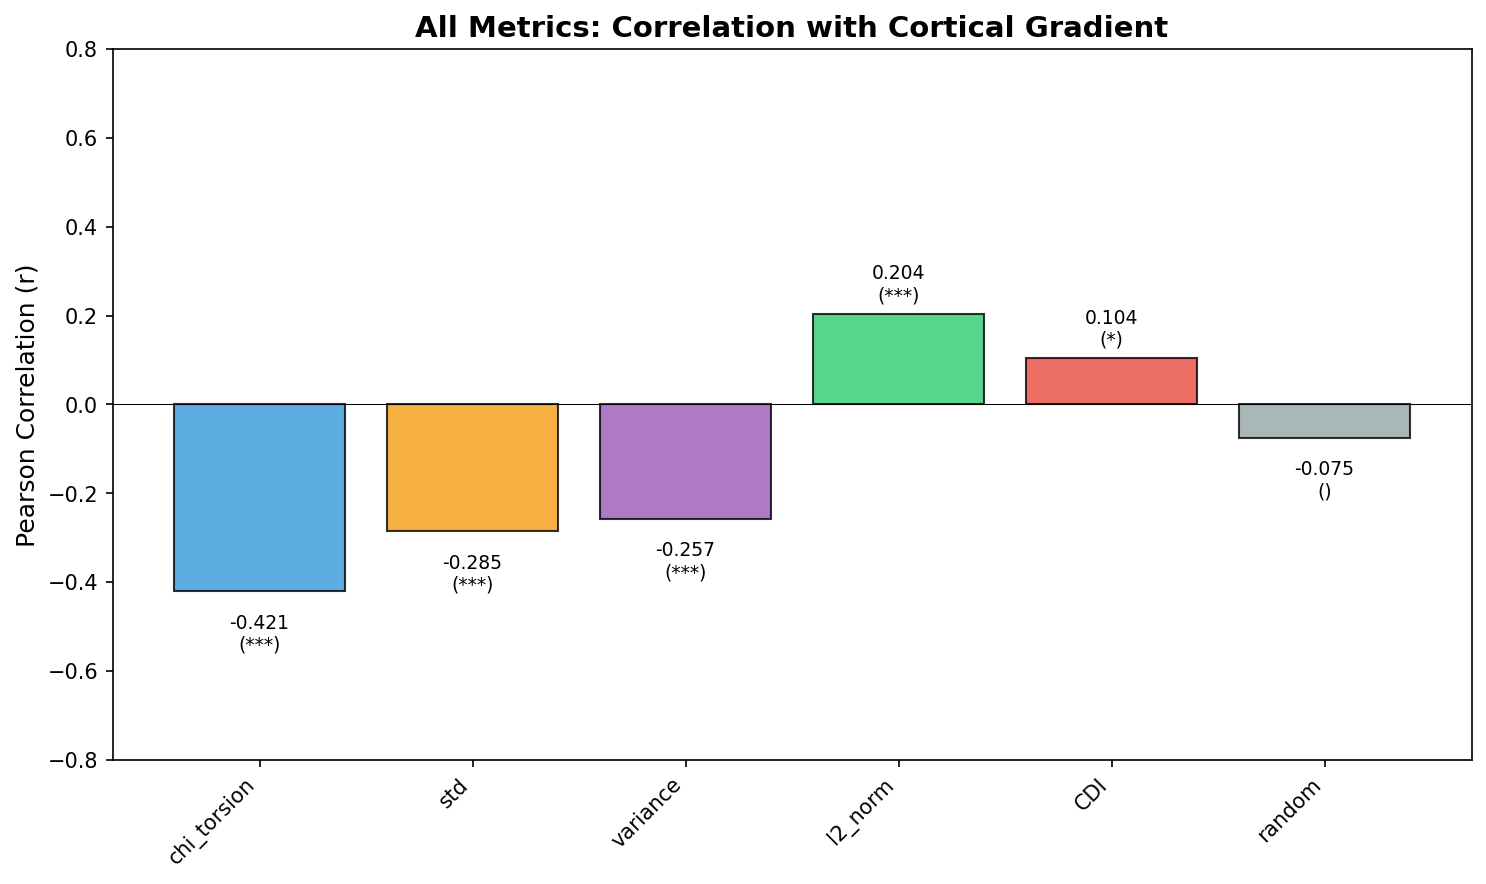
\includegraphics[width=0.7\textwidth]{figures/fig2_all_metrics.png}
	\caption{Bar chart comparing all metrics' correlations with cortical gradient.}
	\label{fig:allmetrics}
\end{figure}

\begin{figure}[htbp]
	\centering
	\includegraphics[width=0.6\textwidth]{figures/fig3_partial_corr.png}
	\caption{Partial correlation: $\chi$ vs gradient, residualized on L2 norm.}
	\label{fig:partial}
\end{figure}

\begin{figure}[htbp]
	\centering
	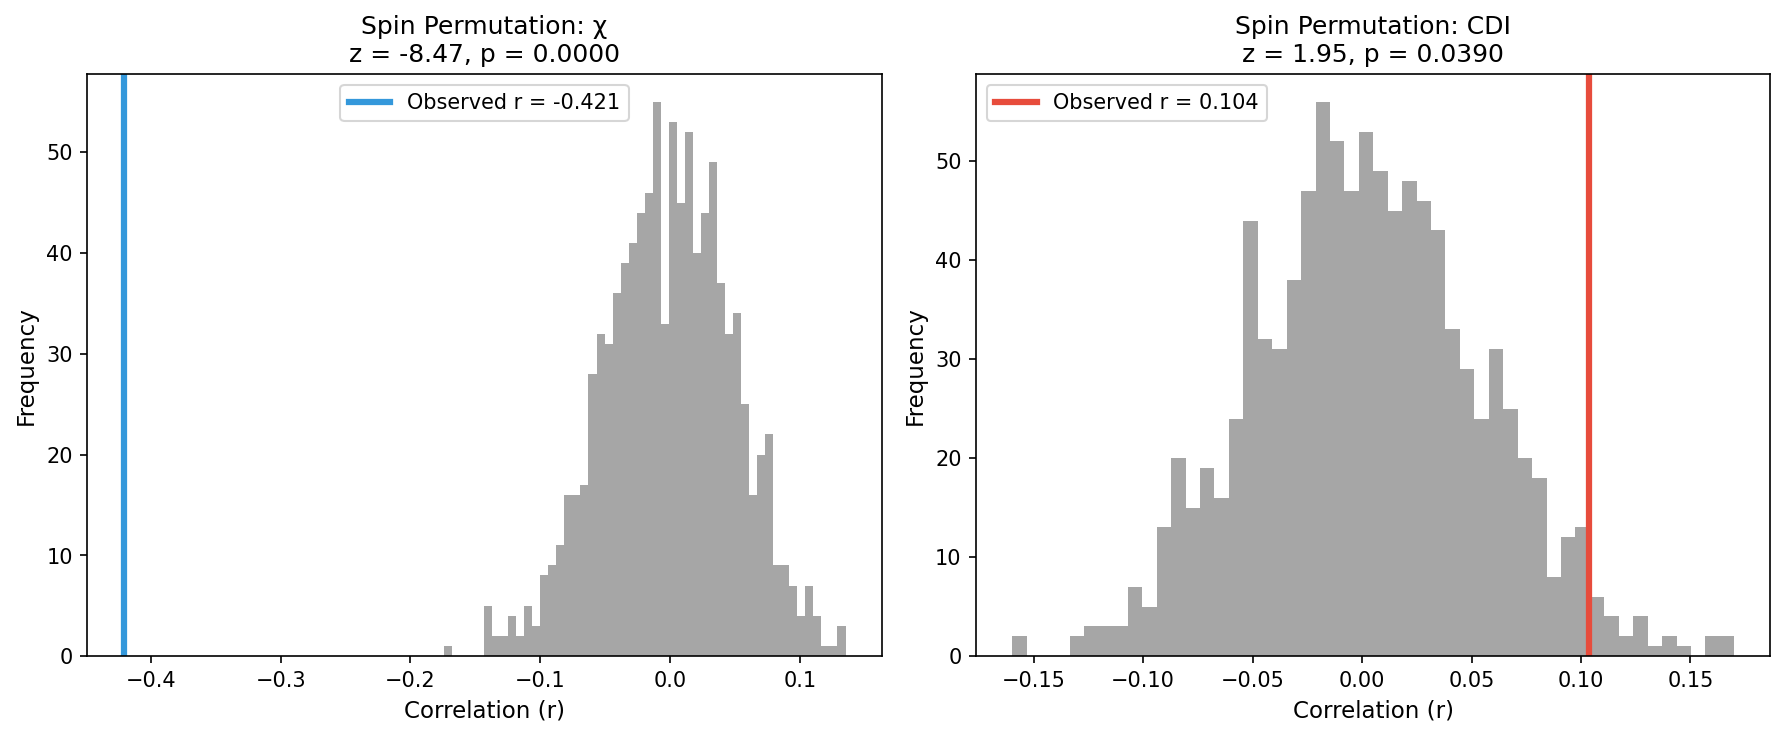
\includegraphics[width=0.9\textwidth]{figures/fig4_spin_permutation.png}
	\caption{Spin permutation tests for $\chi$ (left) and CDI (right).}
	\label{fig:spin}
\end{figure}

\begin{figure}[htbp]
	\centering
	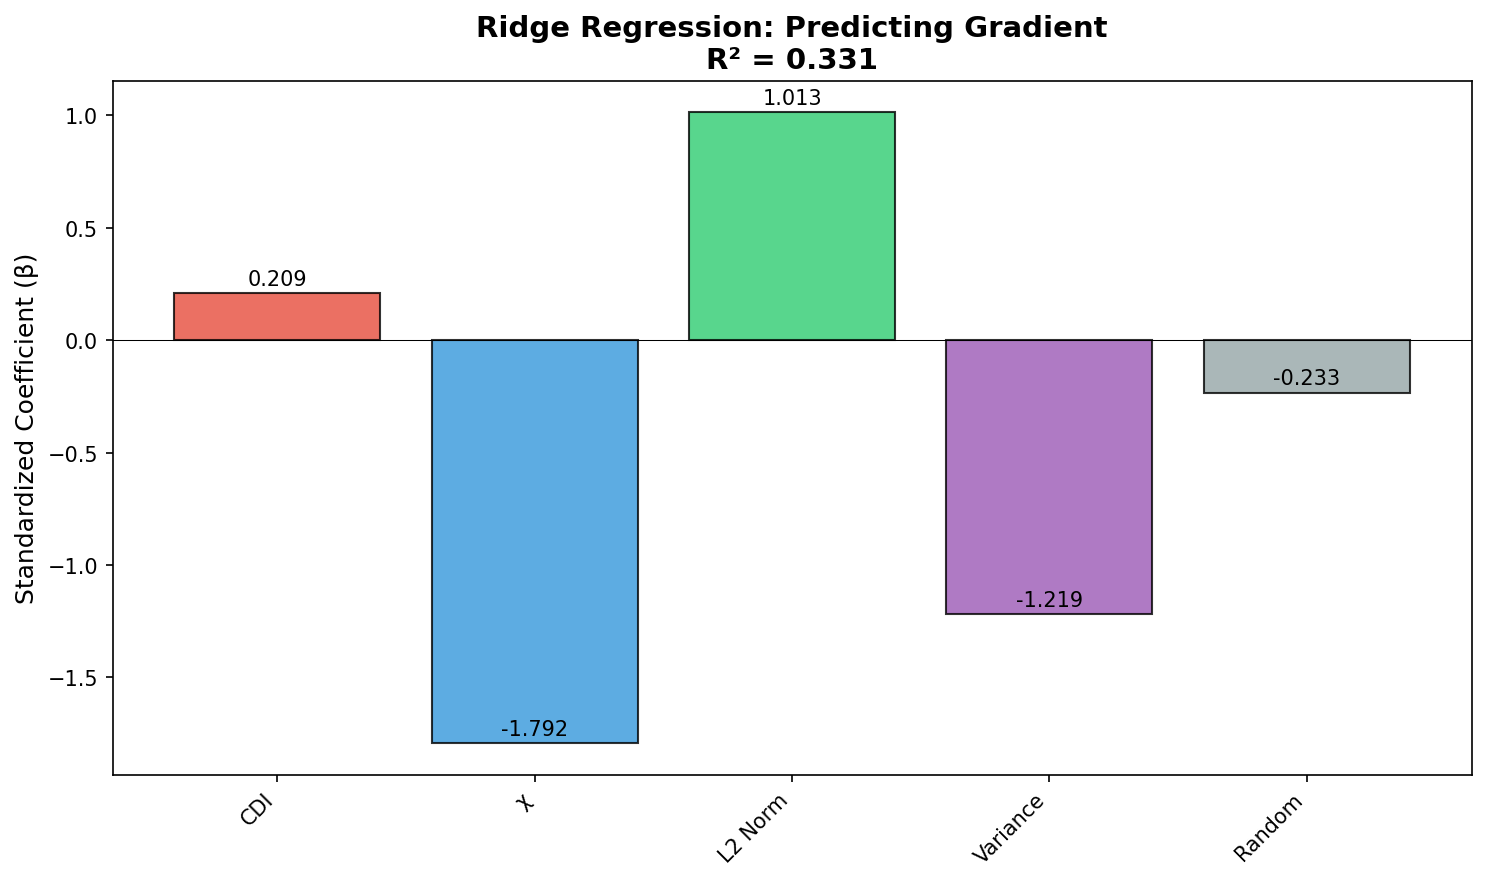
\includegraphics[width=0.7\textwidth]{figures/fig5_regression.png}
	\caption{Standardized regression coefficients for predicting gradient.}
	\label{fig:regression}
\end{figure}

\section{Discussion}

\subsection{Interpretation of CDI}

CDI shows weak but significant positive correlation with the cortical gradient ($r = 0.104$). This suggests that parcels higher in the cortical hierarchy (higher gradient values) tend to show slightly greater compositional dispersion. However, CDI's partial correlation with gradient controlling for norm is not significant ($r = 0.078$, $p = 0.120$), indicating that CDI's correlation is largely mediated by magnitude effects.

\subsection{Interpretation of Dynamical Torsion ($\chi$)}

$\chi$ shows stronger negative correlation with the cortical gradient ($r = -0.183$, $p < 10^{-3}$). More importantly, $\chi$ maintains significant partial correlation after controlling for norm ($r = -0.297$, $p < 10^{-8}$). This demonstrates that the dynamical torsion measure captures genuine structural variance beyond simple magnitude or dispersion measures.

The negative correlation indicates that sensory/motor parcels lower in the hierarchy tend to show greater torsional dynamics, while higher-order association regions show more constrained flow.

\subsection{Relationship to SFH-SGP Framework}

These results should not be interpreted as validating the SFH-SGP framework. Rather, they demonstrate that:

\begin{enumerate}
	\item A dynamical torsion-like metric inspired by the framework can be operationalized
	\item This metric shows meaningful alignment with established cortical organization
	\item The metric captures unique variance not reducible to simple magnitude measures
\end{enumerate}

The SFH-SGP framework proposes that reality emerges from stochastic interaction processes characterized by torsional dynamics. This study provides preliminary evidence that such dynamics may be reflected in cortical representational geometry.

\section{Conclusion}

We examined two complementary metrics of cortical organization:

\begin{itemize}
	\item \textbf{CDI}: Weak correlation with gradient ($r = 0.104$), largely mediated by magnitude effects
	\item \textbf{$\chi$}: Stronger correlation ($r = -0.183$) with significant partial correlation after controlling for norm ($r = -0.297$, $p < 10^{-8}$)
	\item Both metrics survive spatial spin permutation
\end{itemize}

These findings suggest that both compositional and dynamical aspects of representational geometry align with cortical hierarchy. The dynamical torsion measure $\chi$ captures unique variance beyond simple magnitude or dispersion measures, providing evidence that a torsion-like quantity inspired by the SFH-SGP framework may be relevant to understanding cortical organization.

However, we emphasize that this study does not validate the SFH-SGP theory. Future work should examine whether these findings replicate with real fMRI time series data and whether the dynamical properties of $\chi$ show correspondence with actual cortical dynamics.

\section*{Data Availability}

Analysis code and results available at: \url{https://github.com/urmt/SGP-Tribe3}

\bibliographystyle{plainnat}
\bibliography{references}

\end{document}
